\section{From optimal points to optimal motion}
\label{sec:dynamic-question}

The first two parts asked where a given machine should operate and which
machines can support a required set of operating points.  A third problem is
logically independent:
\[
 \boxed{\vect i_A\longrightarrow\gamma(t)\longrightarrow\vect i_B.}
 \tag{25.1}
\]
The fact that both endpoints minimize steady-state loss says nothing about the
best route between them.  A straight interpolation is privileged only when
all current directions have identical speed, there is no drift, and no
intermediate constraint becomes active.  None is generic in a synchronous
drive.  Figure~\ref{fig:dynamic-primer} introduces the required geometry
before any differential-geometric terminology.

\begin{figure}[tb]
\centering
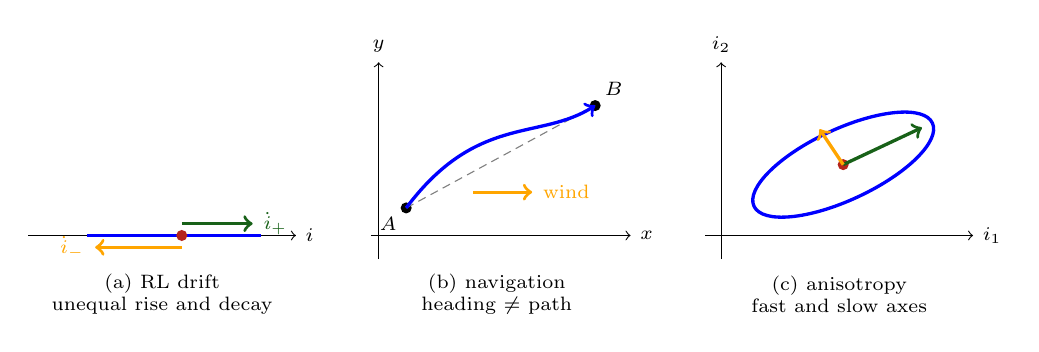
\begin{tikzpicture}[x=1cm,y=1cm,font=\scriptsize]
  \begin{scope}[shift={(0,0)}]
    \draw[->] (-.2,0)--(3.2,0) node[right] {$i$};
    \draw[very thick,blue] (.55,0)--(2.75,0);
    \fill[BrickRed] (1.75,0) circle (2pt);
    \draw[->,ForestGreen!70!black,very thick] (1.75,.15)--(2.65,.15) node[right] {$\dot i_+$};
    \draw[->,Orange,very thick] (1.75,-.15)--(.65,-.15) node[left] {$\dot i_-$};
    \node[align=center] at (1.5,-.75) {(a) RL drift\\unequal rise and decay};
  \end{scope}
  \begin{scope}[shift={(4.25,0)}]
    \draw[->] (-.1,0)--(3.2,0) node[right] {$x$};
    \draw[->] (0,-.3)--(0,2.2) node[above] {$y$};
    \fill (0.35,.35) circle (2pt) node[below left] {$A$};
    \fill (2.75,1.65) circle (2pt) node[above right] {$B$};
    \draw[densely dashed,gray] (.35,.35)--(2.75,1.65);
    \draw[blue,very thick,->] (.35,.35)..controls(1.25,1.55)and(2.05,1.2)..(2.75,1.65);
    \draw[->,Orange,very thick] (1.2,.55)--(1.95,.55) node[right] {wind};
    \node[align=center] at (1.5,-.75) {(b) navigation\\heading $\neq$ path};
  \end{scope}
  \begin{scope}[shift={(8.6,0)}]
    \draw[->] (-.2,0)--(3.2,0) node[right] {$i_1$};
    \draw[->] (0,-.3)--(0,2.2) node[above] {$i_2$};
    \draw[blue,very thick,rotate around={25:(1.55,.9)}] (1.55,.9) ellipse (1.25 and .45);
    \fill[BrickRed] (1.55,.9) circle (2pt);
    \draw[->,ForestGreen!70!black,very thick] (1.55,.9)--(2.55,1.37);
    \draw[->,Orange,very thick] (1.55,.9)--(1.25,1.35);
    \node[align=center] at (1.5,-.75) {(c) anisotropy\\fast and slow axes};
  \end{scope}
\end{tikzpicture}
\caption{Three concrete reasons why Euclidean current interpolation is not a
dynamic optimum: drift, advection, and anisotropic voltage-to-current speed.}
\label{fig:dynamic-primer}
\end{figure}



\subsection{Three elementary models}

For a one-dimensional RL branch with a constant opposing electromotive force
\(e\),
\[
 L\dot i=u-Ri-e,\qquad |u|\leq U,
 \tag{25.2}
\]
the reachable velocity interval is
\[
 \dot i\in\left[\frac{-U-Ri-e}{L},\frac{U-Ri-e}{L}\right].
 \tag{25.3}
\]
It is not centred at zero.  Current rise against \(e\) and decay with the
natural drift therefore need not require the same time.  This already rules
out a symmetric distance whenever drift is significant.

An aircraft with airspeed bound \(\|\vect v\|\leq v_a\) and wind
\(\vect W\) obeys \(\dot{\vect x}=\vect W+\vect v\).  Its ground-velocity
circle is translated by the wind, so the heading is not generally the ground
path.  Zermelo's navigation problem asks for the minimum-time route in exactly
this setting \parencite{zermelo1931,bao2004}.

Finally, if \(\dot{\vect i}=\operatorname{diag}(1/\tau_d,1/\tau_q)\vect u\)
and \(\|\vect u\|\leq1\), the locally attainable current velocities form an
ellipse.  The Euclidean diagonal is not distinguished by the converter; the
fast direction is determined by the ellipse.  These three examples isolate
drift, anisotropy, and direction-dependent speed before they appear together
in the machine.

\subsection{A reciprocal dynamic EESM model}
\label{subsec:dynamic-eesm}

Let the current and voltage vectors be
\[
 \vect i=\begin{bmatrix}i_{\mathrm d}&i_{\mathrm q}&i_{\mathrm f}\end{bmatrix}^{\mathsf T},
 \qquad
 \vect u=\begin{bmatrix}u_{\mathrm d}&u_{\mathrm q}&u_{\mathrm f}\end{bmatrix}^{\mathsf T}.
 \tag{25.4}
\]
Here \(i_{\mathrm f}=i_{\mathrm{exc}}\).  The earlier stationary parameter
\(L_{\mathrm{exc}}i_{\mathrm{exc}}\) describes the stator direct-axis flux
created by the rotor winding.  A dynamic rotor voltage equation additionally
needs the field self inductance and reciprocal mutual coupling.  Under linear,
sinusoidal, rotor-oriented assumptions the energy-consistent flux map is
\[
 \gls{sym:fluxvec}=\matr L\vect i,
 \qquad
 \matr L=
 \begin{bmatrix}
 L_{\mathrm d}&0&L_{\mathrm m}\\
 0&L_{\mathrm q}&0\\
 L_{\mathrm m}&0&L_{\mathrm f}
 \end{bmatrix}=\matr L^{\mathsf T}\succ0.
 \tag{25.5}
\]
Thus \(L_{\mathrm m}=L_{\mathrm{exc}}\) in the stator torque equation, while
\(L_{\mathrm f}\) is a separate rotor self inductance.  Reciprocity follows
from \(\partial\psi_{\mathrm d}/\partial i_{\mathrm f}
=\partial\psi_{\mathrm f}/\partial i_{\mathrm d}=L_{\mathrm m}\), and positive
magnetic coenergy requires
\[
 L_{\mathrm d}>0,\quad L_{\mathrm q}>0,\quad L_{\mathrm f}>0,
 \quad L_{\mathrm d}L_{\mathrm f}-L_{\mathrm m}^2>0.
 \tag{25.6}
\]
The direct--quadrature speed coupling is stored in
\[
 \matr C(\omega_{\mathrm e})=
 \begin{bmatrix}0&-\omega_{\mathrm e}&0\\
 \omega_{\mathrm e}&0&0\\0&0&0\end{bmatrix},
 \qquad
 \matr R_e=\operatorname{diag}(R_{\mathrm s},R_{\mathrm s},R_{\mathrm{exc}}).
 \tag{25.7}
\]
Faraday's law in the rotating frame gives
\[
 \vect u=\matr R_e\vect i+\matr C\gls{sym:fluxvec}
          +\frac{\mathrm d\gls{sym:fluxvec}}{\mathrm dt}.
 \tag{25.8}
\]
For a nonlinear reciprocal map \(\gls{sym:fluxvec}=\gls{sym:fluxvec}(\vect i)\),
\[
 \gls{sym:ldiff}(\vect i):=
 \frac{\partial\gls{sym:fluxvec}}{\partial\vect i},\qquad
 \gls{sym:ldiff}\dot{\vect i}
 =\vect u-\vect r(\vect i,\omega_{\mathrm e}),
 \tag{25.9}
\]
where \(\vect r=\matr R_e\vect i+\matr C\gls{sym:fluxvec}\).  Whenever the
differential inductance is nonsingular,
\[
 \boxed{\dot{\vect i}=\gls{sym:drift}(\vect i,\omega_{\mathrm e})
 +\gls{sym:binput}(\vect i)\vect u},\qquad
 \vect f=-\matr L_{\mathrm{diff}}^{-1}\vect r,quad
 \matr B=\matr L_{\mathrm{diff}}^{-1}.
 \tag{25.10}
\]
This is the dynamic object missing from a stationary current optimization.
For the linear EESM, \(\matr L_{\mathrm{diff}}=\matr L\).  The torque remains
\[
 M=k_{\mathrm T}i_{\mathrm q}
 \bigl((L_{\mathrm d}-L_{\mathrm q})i_{\mathrm d}+L_{\mathrm m}i_{\mathrm f}\bigr).
 \tag{25.11}
\]

\begin{figure}[tb]
\centering
\begin{tikzpicture}[node distance=10mm and 11mm,font=\small]
 \node[draw,rounded corners,fill=blue!8,minimum width=28mm,minimum height=10mm] (u) {converter set $\mathcal U$};
 \node[draw,rounded corners,fill=ForestGreen!10,right=of u,minimum width=31mm,minimum height=10mm] (ld) {$\matr L_{\rm diff}^{-1}$};
 \node[draw,rounded corners,fill=orange!12,right=of ld,minimum width=30mm,minimum height=10mm] (v) {current velocity};
 \node[draw,rounded corners,fill=purple!8,below=of ld,minimum width=34mm,minimum height=10mm] (drift) {$-\matr L_{\rm diff}^{-1}\vect r$};
 \draw[->,thick] (u)--node[above] {$\vect u$}(ld);
 \draw[->,thick] (ld)--node[above] {controlled}(v);
 \draw[->,thick] (drift)-|node[pos=.25,left] {drift}(v);
 \node[draw,align=left,below left=13mm and -2mm of drift,fill=gray!8] (phys)
 {$\vect r=\matr R_e\vect i+\matr C(\omega_e)\boldsymbol\psi$\\resistance $+$ back-EMF $+$ cross coupling};
 \node[draw,align=left,below right=13mm and -2mm of drift,fill=gray!8] (flux)
 {$\boldsymbol\psi(\vect i)$, reciprocal Jacobian\\saturation changes local geometry};
 \draw[->] (phys)--(drift); \draw[->] (flux)--(ld);
\end{tikzpicture}
\caption{The full electrical dynamics separate converter authority, the
differential-inductance map, and natural drift.  Omitting the field-winding
row would remove both a slow state and an independent voltage constraint.}
\label{fig:dynamic-model}
\end{figure}



The PSM is the two-state teaching slice with
\(\boldsymbol\psi_s=[L_{\mathrm d}i_{\mathrm d}+\psi_{\mathrm{pm}},
L_{\mathrm q}i_{\mathrm q}]^{\mathsf T}\).  It has no controllable rotor
winding, and the PM offset enters the drift through \(\matr C\boldsymbol\psi_s\).
It is therefore not obtained by setting \(R_{\mathrm{exc}}=0\).

\subsection{Fixed speed first, mechanical speed second}

For an electrical transient short compared with the mechanical time scale,
\(\omega_{\mathrm e}\) is treated as a measured constant.  Sections
\ref{sec:velocity-geometry}--\ref{sec:fast-slow-experiment} solve and interpret
that case.  If speed changes materially, augment the state by
\(\omega_{\mathrm m}\) and add
\[
 J\dot\omega_{\mathrm m}=M-M_L-B_m\omega_{\mathrm m},
 \qquad \omega_{\mathrm e}=p\omega_{\mathrm m}.
 \tag{25.12}
\]
The current velocity body then changes with the mechanical state; a path in
three-current space is only the projection of a four-dimensional trajectory.

